


\begin{table}
{\scriptsize
\begin{center}
\begin{tabular}{|c||c|c|c|c|c||c|c|c|c|c|}
\hline
\hline
& \multicolumn{3}{|c|}{Program Source} & \multicolumn{1}{|c|}{Test Suite} \\
\hline
Subject & \#Classes. & \#Methods & SLOC & \#Test cases \\
\hline
\hline
{\tt Apache Commons} & & & & \\
{\tt Validator} & 64 & 578 & 6,033 & 434 \\
\hline
{\tt JExel 1.0.0} & & & & \\
{\tt beta 13} & 43 & 133 & 1,522	 & 344  \\
\hline
{\tt JAxen} & 167 & 1,078 & 12,462 & 2,138\\
\hline
{\tt JParser} & 115 & 178 & 3,046 & 647 \\
\hline
{\tt Apache Commons} & & & & \\
{\tt CLI} & 23 & 208 & 2,667 & 364 \\ 
\hline
\hline
\end{tabular}
\end{center}
}
\caption{Open Source Subject Programs}
\label{tab:opensourcesubs}
\end{table}



The SIR results show that reduction is useful for localization in an
idealized setting where suites are relatively complete and faults are
chosen for certain properties, and the Spidermonkey results show its
value in a particularly challenging setting (where passing tests have
very wide-ranging coverage).  How does reduction affect localization
in a typical open source project?

We attempted to answer this question by picking five open source Java
programs (shown in Table \ref{tab:opensourcesubs}) and generating mutants for each of the project to simulate bugs as it is commonly done in recent fault localization literature.\cite{mutant} \cite{PureTest}



\begin{figure}[t]
  \centering
  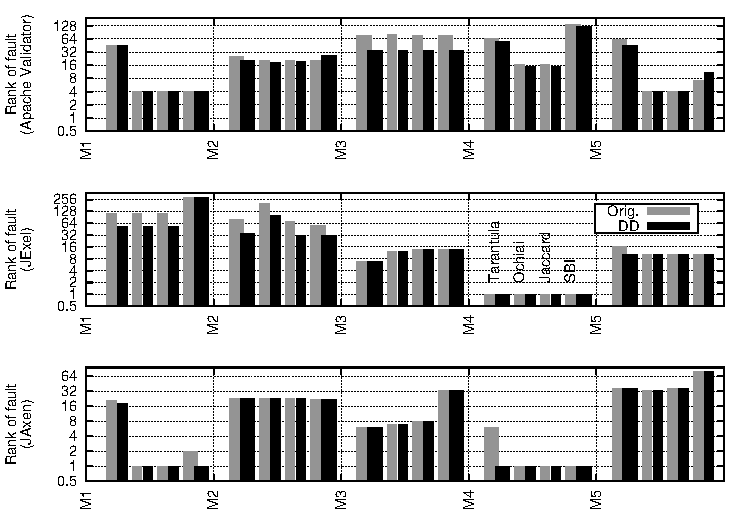
\includegraphics[width=\columnwidth]{opensource1}
  \caption{First Set of Open Source Results}
  \label{fig:opensource1}
\end{figure}

\begin{figure}[t]
  \centering
  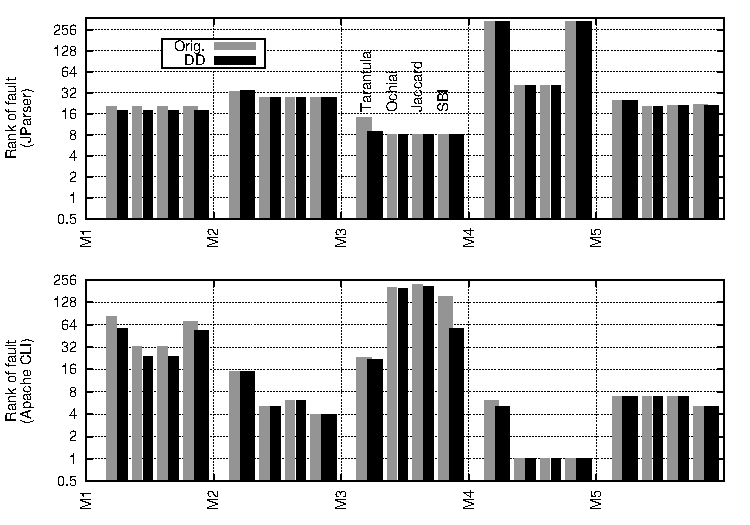
\includegraphics[width=\columnwidth]{opensource2}
  \caption{Second Set of Open Source Results}
  \label{fig:opensource2}
\end{figure}

 
Our strategy was to create mutants in the same way as Xuan and
Monperrus \cite{PureTest} in their own localization work, using 6
mutant operators.  From each set of mutants generated, we selected 5
or 6 mutants at random that met the following criteria: (1) the mutant
was killed by at least one test case and (2) the mutant generated no
errors in JUnit test cases.  A JUnit failure is caused by an
unsatisfied assertion, but an error is caused by another kind of test
failure, which may include some test setup or oracle problems.  Using
assertion failures only assures that we were remaining within the
intent of the original tests.

Figures \ref{fig:opensource1} and \ref{fig:opensource2} show the
results of applying reduction to these simulated faults.  Taking all
the open source projects and mutants together, we note that reduction
improved fault ranking in 51 cases, left it unchanged in 55 cases, and
made it worse in 2 cases.  The average improvement was 17.62 ranking
positions; the average negative effect size was 2 ranking positions.
The best improvement was 100
rank positions.  The average fault ranking without
reduction was 37.64 and with reduction it improved to 29.36.  